\chapter{Lux.jl: Bridging Scientific Computing and Deep Learning}
\label{chapter:lux_bridging_scientific_computing_and_deep_learning}

\section{Introduction}
\label{sec:introduction_lux}

Julia already has quite a few well established Neural Network Frameworks – Flux~\citep{innes2018fashionable} \& KNet~\citep{yuret2016knet}. However, certain design elements – \textit{Coupled Model and Parameters} \& \textit{Internal Mutations} – associated with these frameworks make them less compiler and user friendly. Making changes to address these problems in the respective frameworks would be too disruptive for users. In this chapter, we introduce Lux: a neural network framework built completely using pure functions to make it both compiler and autodiff friendly.

The main design principles of Lux include:
%
\begin{enumerate}
  \item \textit{Truly Immutable Models} storing information to construct a layer rather than the parameters and states.
  \item All models are \textit{pure functions} and outputs are completely \textit{deterministic} given the inputs.
  \item Models are decoupled from the parameters and states. This allows us to \textit{perform easy parameter manipulation} like in \textit{Weight Normalization}, \textit{Hypernetworks} and \textit{Spectral Normalization}.
\end{enumerate}
%

\section{Composability via Generic Parameterization}
\label{sec:composability}

One of the distinguishing features of Lux.jl is its generic parameters interface. Lux can accept any special parameter type as long as the parameters are accessible via \textit{getproperty}. This allows Lux to seamlessly interface with packages that are completely agnostic to the specifics of Lux. This is in contrast to most prior works that require glue code for interfacing -- like Flux.jl~\citep{innes:2018} -- or requires reimplementing algorithms in specific Domain Specific Languages (DSLs) -- like Pytorch~\citep{paszke2019pytorch,paszke2017automatic}, JAX~\citep{jax2018github}, Tensorflow~\citep{tensorflow2015-whitepaper}.

Scientific Computing softwares differ from most modern ML softwares in that they are designed to operate on arrays, while ML softwares operate on deeply nested structures. This is a fundamental difference that makes it difficult to interface between the two. However, Lux.jl is designed to be agnostic to the underlying data structure. In this section, we will demonstrate several examples interfacing Lux with Scientific Computing frameworks solving Neural ODEs, Physics Informed Neural Networks and Optimization Problems.

\subsection{Neural Differential Equations}
\label{subsec:differential_equations_lux}

In this thesis, we have described Neural ODEs in great depth. However, for physics based modelling we often need to rely on higher order differential equations. In this section, we will describe how to model a second order differential equation using Lux.jl and OrdinaryDiffEq.jl. We will attempt to model the acceleration of a system using a Neural Network\footnote{We have modified this example from \url{https://docs.sciml.ai/SciMLSensitivity/stable/examples/ode/second_order_neural/}}:
%
\begin{equation}
  \frac{d^2u}{dt^2} = \texttt{NN}(u)
\end{equation}
%

\inputminted[linenos, breaklines, fontsize=\scriptsize, frame=single, framesep=10pt]{julia}{../code/diffeq.jl}

\begin{figure}
  \centering
  \begin{subfigure}[c]{0.48\linewidth}
    \centering
    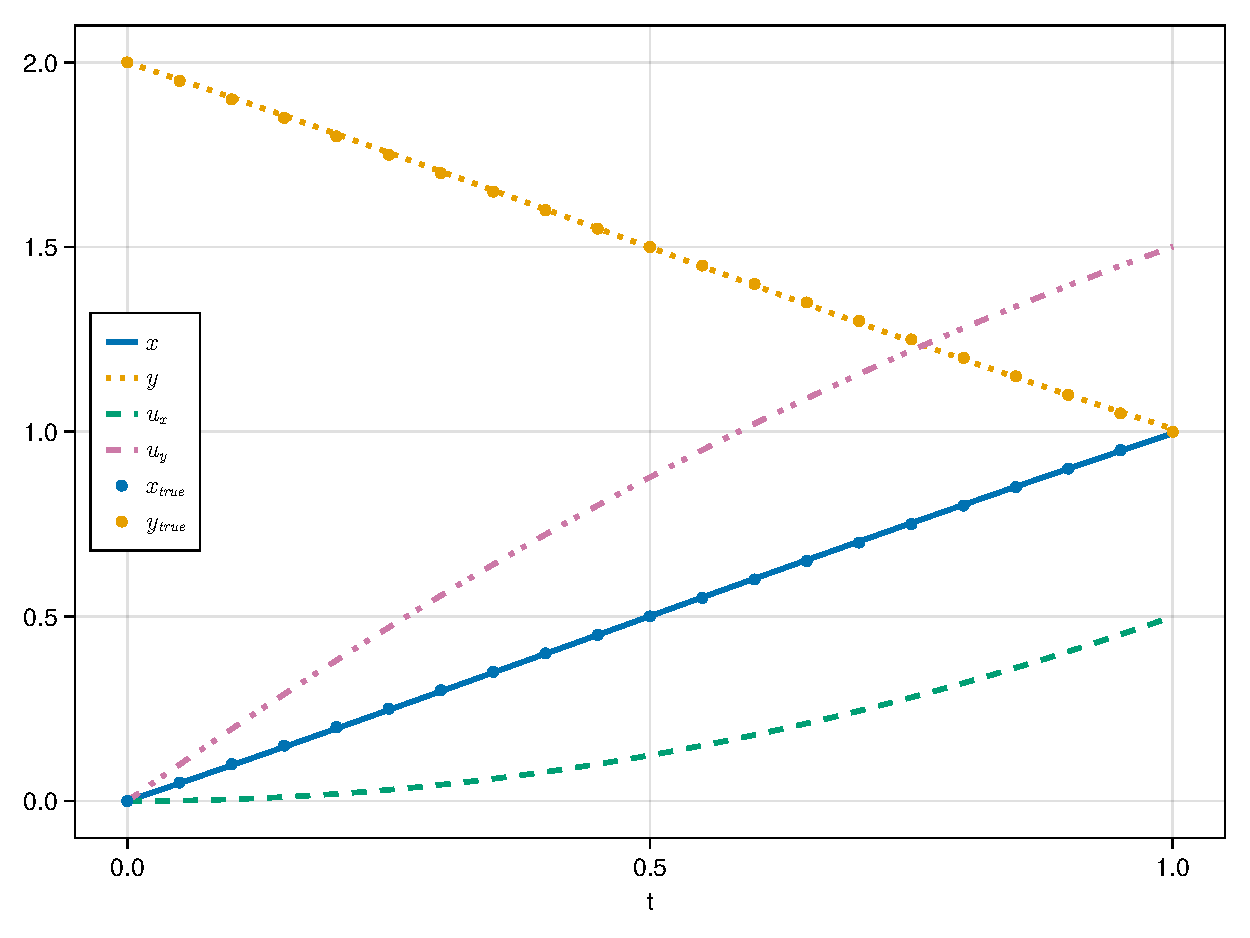
\includegraphics[width=\textwidth]{../figures/lux/diffeq_plot.pdf}
    \caption{\textbf{Learning $2^{nd}$ order differential equation with Lux.jl.}}
    \label{fig:lux_diffeq_plot}
  \end{subfigure}
  \hfill
  \begin{subfigure}[c]{0.48\linewidth}
    \centering
    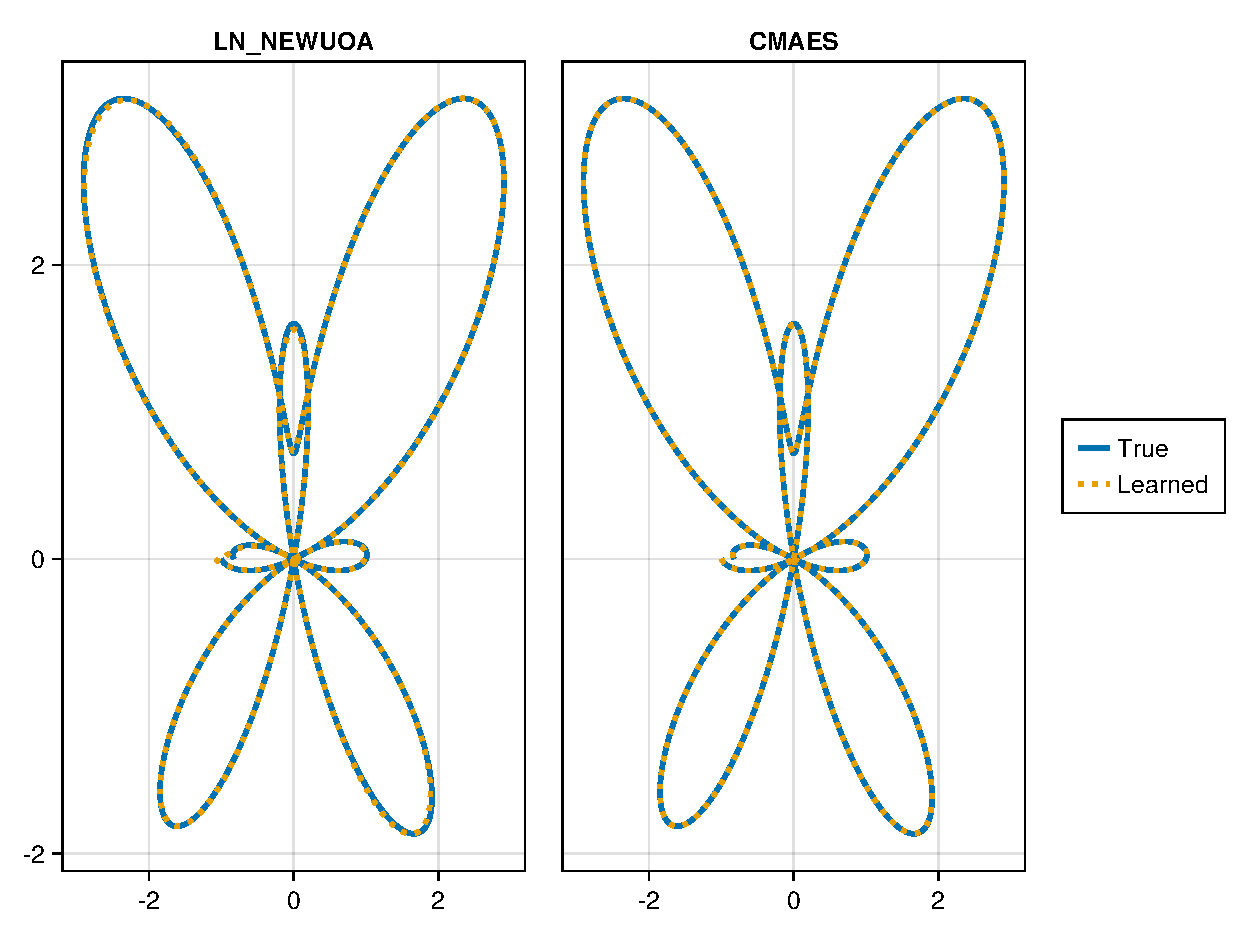
\includegraphics[width=\textwidth]{../figures/lux/gfopt_plot.pdf}
    \caption{\textbf{Gradient Free Optimization to train a neural network} to approximate the function $r(\theta) = e^{sin(\theta)} - 2cos(4\theta) + sin\left(\frac{2\theta - \pi}{12}\right)^5$.}
    \label{fig:lux_gfopt_plot}
  \end{subfigure}
\end{figure}

% \begin{figure}[t]
%   \centering
%   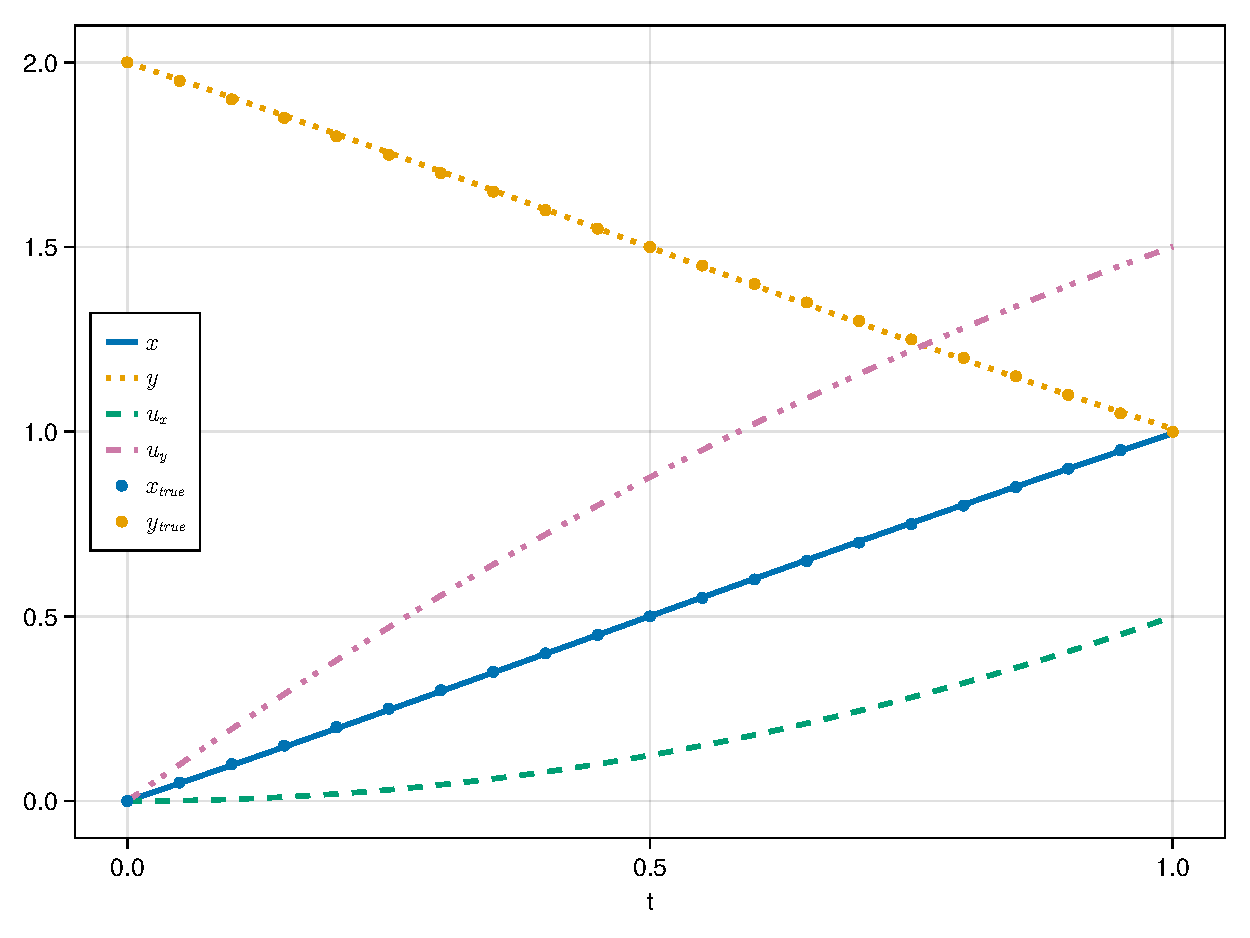
\includegraphics[width=0.5\textwidth]{../figures/lux/diffeq_plot.pdf}
%   \caption{\textbf{Learning $2^{nd}$ order differential equation with Lux.jl.}}
%   \label{fig:lux_diffeq_plot}
% \end{figure}

\Cref{fig:lux_diffeq_plot} shows that our model is able to accurately learn the dynamics of the system from a few discrete data points. This is a very simple example, but it demonstrates the composability of Lux.jl and DifferentialEquations ecosystem.

\subsection{Gradient Free Optimization Algorithms}
\label{subsec:evolutionary_alg_lux}

Lux allows the parameters of a complicated neural network to be represented as a flattened vector. This allows it to interface directly with optimization packages without any glue code. In this example, we will train a neural network with gradient-free optimization algorithms to learn the function:
%
\begin{align}
  r(\theta)              & = e^{sin(\theta)} - 2cos(4\theta) + sin\left(\frac{2\theta - \pi}{12}\right)^5 \\
  \texttt{where } \theta & \in [0, 2\pi]
\end{align}
%
We will use algorithms implemented in packages that are agnostic to the specifics of Lux\footnote{Note that these are not the most efficient algorithms to solve the problem, but these simply demonstrate the composability of Lux.}:
%
\begin{itemize}
  \item Covariance Matrix Adaptation Evolutionary Strategy (CMAES)~\citep{hansen2016cma} from CMAEvolutionStrategy.jl.
  \item LN\_NEWUOA~\citep{powell2006newuoa} from NLopt.jl~\citep{johnson2021nlopt}. Since Lux allows flattened parameters we can easily interoperate with NLopt which is a C library.
\end{itemize}
%

\inputminted[linenos, breaklines, fontsize=\scriptsize, frame=single, framesep=10pt]{julia}{../code/gfopt.jl}

% \begin{figure}[t]
%   \centering
%   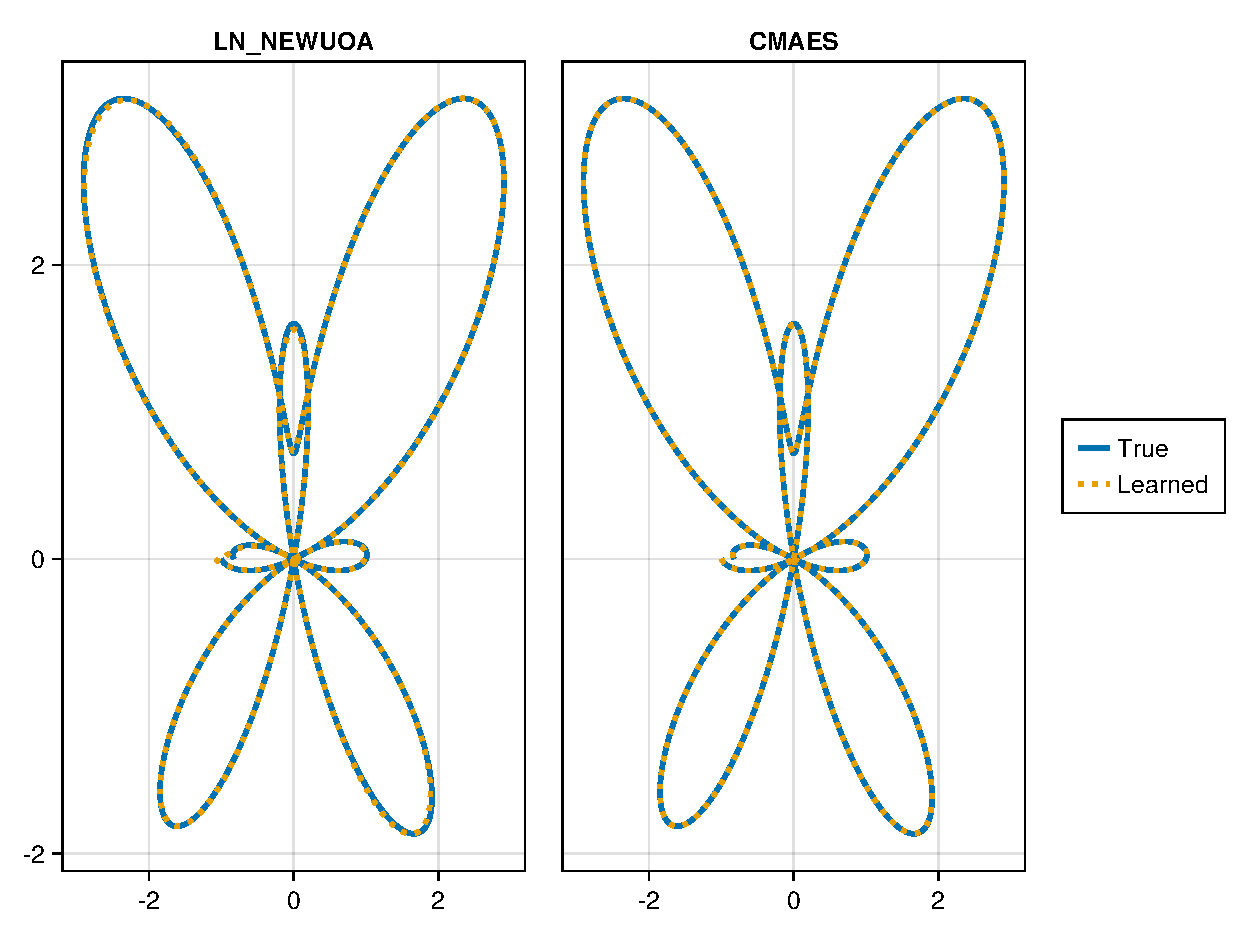
\includegraphics[width=0.8\textwidth]{../figures/lux/gfopt_plot.pdf}
%   \caption{\textbf{Gradient Free Optimization to train a neural network} to approximate the function $r(\theta) = e^{sin(\theta)} - 2cos(4\theta) + sin\left(\frac{2\theta - \pi}{12}\right)^5$.}
%   \label{fig:lux_gfopt_plot}
% \end{figure}

\subsection{Physics Informed Neural Networks}
\label{subsec:physics_informed_neural_networks_lux}

Lux.jl supports PINNs using NeuralPDE.jl~\citep{zubov2021neuralpde}. In this example, we will solve the Kuramoto–Sivashinsky equation\footnote{This example has been adapted from \url{https://docs.sciml.ai/NeuralPDE/stable/examples/ks/}}:
%
\begin{align}
  \frac{\partial \func{u}{x, t}}{\partial t} + \func{u}{x, t} \cdot \frac{\partial \func{u}{x, t}}{\partial x} + \alpha \cdot \frac{\partial^2 \func{u}{x, t}}{\partial x^2} + \beta \cdot \frac{\partial^3 \func{u}{x, t}}{\partial x^3}  + \gamma \cdot \frac{\partial^4 \func{u}{x, t}}{\partial x^4} = 0
\end{align}
%
For $\alpha = \gamma = 1$ and $\beta = 4$, we have the exact analytic solution:
%
\begin{align}
   & \func{u_e}{x, t} = 11 + 15 \tanh \theta - 15 \tanh^2 \theta - 15 \tanh^3 \theta \\
   & \texttt{where } \theta = t - \frac{x}{2}
\end{align}
%
The initial and boundary conditions are given by:
%
\begin{align}
   & \func{u}{x, 0} = \func{u_e}{x, 0}                                                             \\
   & \func{u}{-10, t} = \func{u_e}{-10, t}                                                         \\
   & \func{u}{10, t} = \func{u_e}{10, t}                                                           \\
   & \func{\frac{\partial u}{\partial x}}{-10, t} = \func{\frac{\partial u_e}{\partial t}}{-10, t} \\
   & \func{\frac{\partial u}{\partial x}}{10, t} = \func{\frac{\partial u_e}{\partial t}}{10, t}
\end{align}
%

\begin{figure}[t]
  \centering
  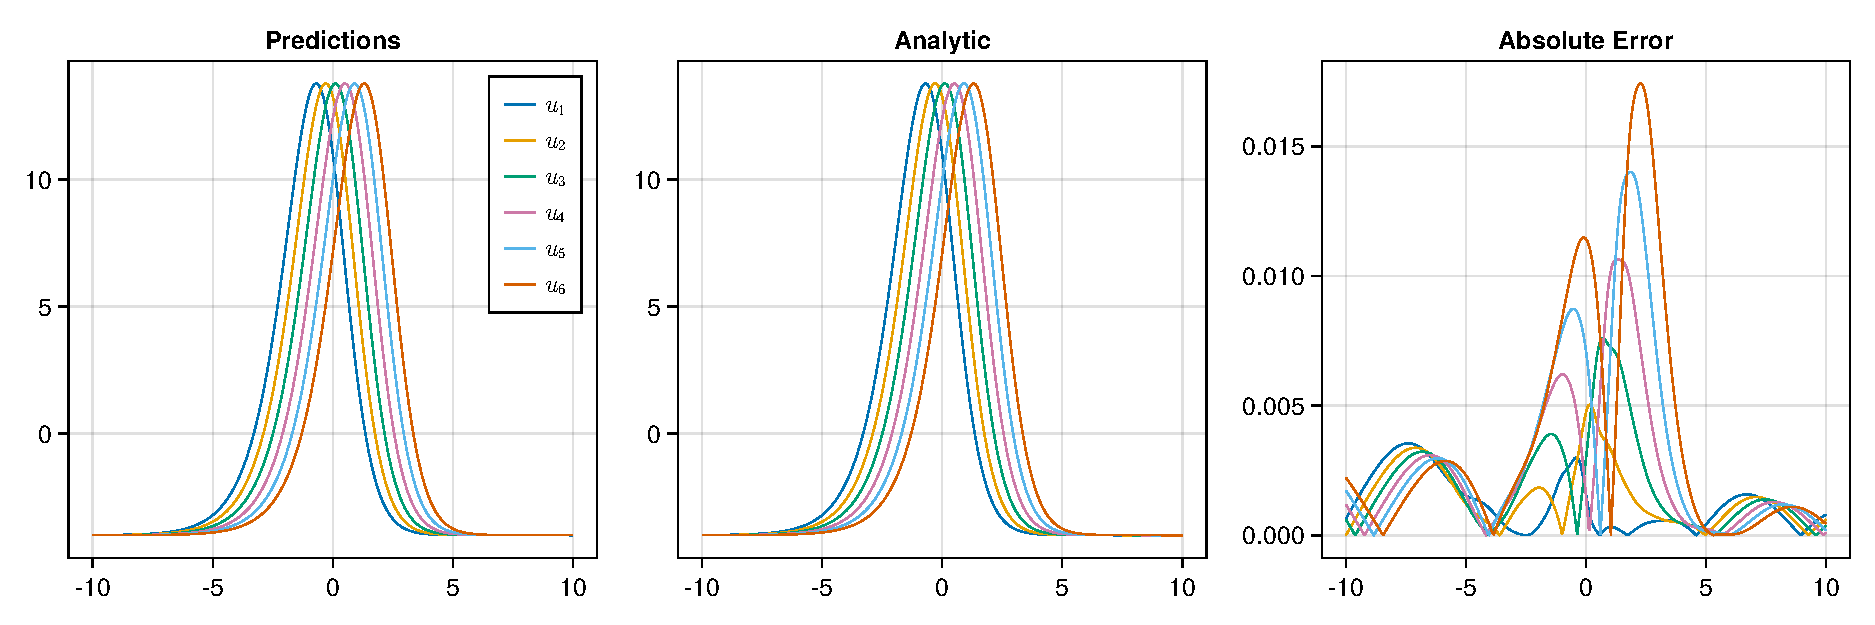
\includegraphics[width=\textwidth]{../figures/lux/pinn_plot.pdf}
  \caption{\textbf{Physics Informed Neural Networks using Lux} for solving Kuramoto–Sivashinsky equation.}
  \label{fig:lux_pinn_plot}
\end{figure}

\inputminted[linenos, breaklines, fontsize=\scriptsize, frame=single, framesep=10pt]{julia}{../code/pinn.jl}

\Cref{fig:lux_pinn_plot} demonstrates that our PINN can solve the Kuramoto–Sivashinsky equation with high accuracy.

\section{Discussion}
\label{sec:discussion_lux}

In this chapter, we have introduced a new neural network framework in Julia. We designed the framework to be modular and composable. We demonstrated the composability of Lux.jl by showing how it can be used with other packages in the Julia ecosystem. We also showed that Lux.jl can be used to solve a variety of problems. Despite being in early days of development, Lux.jl is already being used extensively in research projects and being extended by the open-source community.

\subsection{Current Limitations}
\label{subsec:current_limitations}

Lux.jl has the following known limitations, most of which are being actively worked upon:
%
\begin{itemize}
  \item Lux.jl is not the fastest framework for training small neural networks on CPU. For smaller architectures, \href{https://github.com/PumasAI/SimpleChains.jl}{SmallChains.jl} is the fastest option.
  \item Lux.jl shares the same backend as Flux.jl and hence migration from Flux to Lux doesn't speed up user code. However, a new backend \href{https://github.com/LuxDL/LuxLib.jl}{LuxLib.jl} is under development which should be faster than Flux.jl's backend.
  \item Lux.jl is currently tested to work on CPU and NVIDIA CUDA GPUs. Support for AMD GPUs is being worked upon.
  \item Nested Reverse Mode differentiation of Lux models is not supported yet.
\end{itemize}
%
